% answers.tex —— 2018 年·全国Ⅰ卷·文科 · 参考答案与详细解析片段
% 由 tools/generate_projects.py 依来源总账自 2018/2018_数学真题_文_试题.md + 2018/2018_数学真题_文_解析正文.md + 2018/2018_数学真题_文_答案要点.md 生成，勿手改（改源 MD 后重跑）


\begin{gknotice}
\textbf{ 解析归属声明}：本文解析由本库编写者根据试题\textbf{独立推导}，\textbf{非官方标准答案}。若与官方发布版本不一致，以官方为准。

\textbf{ 卷种提示}：本卷为文理分科时代的旧结构，含\textbf{现已取消}的选做题（第 22/23 题）与\textbf{已删除}的三视图考点（第 9 题）。

\textbf{重合题说明}：第 2、3、6、7、9、14 题及第 22、23 题与同年理科卷完全相同，本文给出结论与要点，完整推导请见理科卷。
\end{gknotice}

\par\medskip

\gkpart{一、选择题}

\begin{answer}
\gksolhead{1}{集合的交}

\textbf{题目}：

已知集合 $A=\{0,2\}$，$B=\{-2,-1,0,1,2\}$，则 $A\cap B=$\mbox{（　　）}

\begin{gkopts}(2)
\task A．$\{0,2\}$
\task B．$\{1,2\}$
\task C．$\{0\}$
\task D．$\{-2,-1,0,1,2\}$
\end{gkopts}

\Needspace{4\baselineskip}
\textbf{解析}

$A$ 的两个元素 $0$ 和 $2$ 都属于 $B$，即 $A\subseteq B$。子集与母集的交集就是子集本身：

\nopagebreak[4]
\[A\cap B=A=\{0,2\}\]

\gkanswer{答案：A（$\{0,2\}$）}

\par\medskip

\end{answer}
\begin{answer}
\gksolhead{2}{复数运算}

\textbf{题目}：

设 $z=\dfrac{1-\mathrm i}{1+\mathrm i}+2\mathrm i$，则 $|z|=$\mbox{（　　）}

\begin{gkopts}(4)
\task A．$0$
\task B．$\dfrac12$
\task C．$1$
\task D．$\sqrt2$
\end{gkopts}

\textbf{解析}（同理科卷第 1 题）

\nopagebreak[4]
\[\frac{1-\mathrm i}{1+\mathrm i}=\frac{(1-\mathrm i)^{2}}{(1+\mathrm i)(1-\mathrm i)}=\frac{-2\mathrm i}2=-\mathrm i\]

故 $z=-\mathrm i+2\mathrm i=\mathrm i$，$|z|=1$。

\gkanswer{答案：C（$1$）}

\par\medskip

\end{answer}
\begin{answer}
\gksolhead{3}{饼图与总量变化}

\textbf{题目}：

某地区经过一年的新农村建设，农村的经济收入增加了一倍，实现翻番。为更好地了解该地区农村的经济收入变化情况，统计了该地区新农村建设前后农村的经济收入构成比例，得到如下饼图：
\nopagebreak[4]
\begin{center}% 2018 全国Ⅰ卷 理3/文3：新农村建设前后经济收入构成比例（双饼图）
% 从 90° 起顺时针切分；标签放各扇区中线角上，小扇区标签外置并加引线
\begin{tikzpicture}[font=\footnotesize, scale=1.0]
  % ---------- 左：建设前（种植60 养殖30 三产6 其他4）----------
  \begin{scope}
    \draw (0,0) circle (1.7);
    \foreach \a in {90, -126, -234, -255.6} {\draw (0,0) -- (\a:1.7);}
    \node at (-18:0.95)  {\shortstack{种植收入\\ $60\%$}};
    \node at (-180:0.95) {\shortstack{养殖收入\\ $30\%$}};
    \draw (-244.8:1.6) -- (-244.8:2.0);
    \node at (-244.8:2.05) [above left, inner sep=1pt] {第三产业收入 $6\%$};
    \draw (-262.8:1.6) -- (-262.8:2.0);
    \node at (-262.8:2.05) [above right, inner sep=1pt] {其他收入 $4\%$};
    \node at (0,-2.15) {\small 建设前经济收入构成比例};
  \end{scope}
  % ---------- 右：建设后（种植37 养殖30 三产28 其他5）----------
  \begin{scope}[xshift=6.2cm]
    \draw (0,0) circle (1.7);
    \foreach \a in {90, -43.2, -151.2, -252} {\draw (0,0) -- (\a:1.7);}
    \node at (23.4:0.95)   {\shortstack{种植收入\\ $37\%$}};
    \node at (-97.2:0.95)  {\shortstack{养殖收入\\ $30\%$}};
    \node at (-201.6:0.92) {\shortstack{第三产业\\ 收入 $28\%$}};
    \draw (-261:1.6) -- (-261:2.0);
    \node at (-261:2.05) [above, inner sep=1.5pt] {其他收入 $5\%$};
    \node at (0,-2.15) {\small 建设后经济收入构成比例};
  \end{scope}
\end{tikzpicture}
\end{center}
\nopagebreak[4]
则下面结论中\textbf{不正确}的是\mbox{（　　）}

\begin{gkopts}(1)
\task A．新农村建设后，种植收入减少
\task B．新农村建设后，其他收入增加了一倍以上
\task C．新农村建设后，养殖收入增加了一倍
\task D．新农村建设后，养殖收入与第三产业收入的总和超过了经济收入的一半
\end{gkopts}

\par\medskip

\Needspace{0.4\textheight}

\textbf{解析}（同理科卷第 3 题）

\textbf{核心陷阱}：饼图给的是\textbf{比例}，而总量翻了一番，比例下降不等于金额下降。设建设前总收入为 $a$，建设后为 $2a$：

\begin{center}
\begin{tabular}{lccl}
\toprule
项目 & 建设前 & 建设后 & 变化 \\
\midrule
种植 & $0.6a$ & $0.37\times2a=0.74a$ & \textbf{增加} \\
养殖 & $0.3a$ & $0.30\times2a=0.60a$ & 恰好翻倍 \\
其他 & $0.04a$ & $0.05\times2a=0.10a$ & 增加 $1.5$ 倍 \\
\bottomrule
\end{tabular}
\end{center}

\begin{itemize}
\item \textbf{A}：种植收入实为增加 → \textbf{不正确}（本题选这个）；
\item B、C、D 经上表核对均正确（D 项 $28\%+30\%=58\%>50\%$）。
\end{itemize}

\gkanswer{答案：A（种植收入减少 —— 这条不正确）}

\par\medskip

\end{answer}
\begin{answer}
\gksolhead{4}{椭圆离心率}

\textbf{题目}：

已知椭圆 $C:\dfrac{x^{2}}{a^{2}}+\dfrac{y^{2}}4=1$ 的一个焦点为 $(2,0)$，则 $C$ 的离心率为\mbox{（　　）}

\begin{gkopts}(2)
\task A．$\dfrac13$
\task B．$\dfrac12$
\task C．$\dfrac{\sqrt2}2$
\task D．$\dfrac{2\sqrt2}3$
\end{gkopts}

\Needspace{4\baselineskip}
\textbf{解析}

\textbf{第一步：判断焦点位置。} 焦点 $(2,0)$ 在 $x$ 轴上，说明\textbf{长轴在 $x$ 轴上}，即 $a^{2}>4$，且

\nopagebreak[4]
\[c=2\]

\textbf{第二步：用 $a^{2}=b^{2}+c^{2}$。} 这里 $b^{2}=4$：

\nopagebreak[4]
\[a^{2}=4+2^{2}=8\ \Longrightarrow\ a=2\sqrt2\]

\textbf{第三步：求离心率。}

\nopagebreak[4]
\[e=\frac ca=\frac2{2\sqrt2}=\frac1{\sqrt2}=\frac{\sqrt2}2\]

\begin{gktip}
\textbf{方法提示}：椭圆题第一件事永远是\textbf{看焦点在哪个轴上}，这决定了 $a^{2}$ 是分母中较大的那个还是较小的那个。本题若误判成焦点在 $y$ 轴，会得到 $a^{2}=4-4=0$ 的荒谬结果。
\end{gktip}

\gkanswer{答案：C（$\dfrac{\sqrt2}2$）}

\par\medskip

\end{answer}
\begin{answer}
\gksolhead{5}{圆柱的轴截面与表面积}

\textbf{题目}：

已知圆柱的上、下底面的中心分别为 $O_1$，$O_2$，过直线 $O_1O_2$ 的平面截该圆柱所得的截面是面积为 $8$ 的正方形，则该圆柱的表面积为\mbox{（　　）}

\begin{gkopts}(4)
\task A．$12\sqrt2\pi$
\task B．$12\pi$
\task C．$8\sqrt2\pi$
\task D．$10\pi$
\end{gkopts}

\Needspace{4\baselineskip}
\textbf{解析}

\textbf{第一步：认识轴截面。} 过轴 $O_1O_2$ 的平面截圆柱，截面是一个矩形，其\textbf{宽等于底面直径 $2r$，高等于圆柱的高 $h$}。

\textbf{第二步：由"正方形"定尺寸。} 正方形要求 $2r=h$，面积为 $8$：

\nopagebreak[4]
\[(2r)^{2}=8\ \Longrightarrow\ 2r=2\sqrt2\ \Longrightarrow\ r=\sqrt2,\quad h=2\sqrt2\]

\textbf{第三步：套表面积公式}（两个底面 $+$ 侧面）：

\nopagebreak[4]
\[S=2\pi r^{2}+2\pi rh=2\pi\times2+2\pi\times\sqrt2\times2\sqrt2=4\pi+8\pi=12\pi\]

\begin{gktip}
\textbf{方法提示}：圆柱侧面积 $2\pi rh$ 的记法是"\textbf{底面周长 $\times$ 高}"，因为侧面展开就是一个 $2\pi r$ 宽、$h$ 高的矩形。本题的干扰项 $12\sqrt2\pi$ 是把 $r$ 与 $2r$ 弄混的结果。
\end{gktip}

\gkanswer{答案：B（$12\pi$）}

\par\medskip

\end{answer}
\begin{answer}
\gksolhead{6}{奇函数与切线}

\textbf{题目}：

设函数 $f(x)=x^{3}+(a-1)x^{2}+ax$。若 $f(x)$ 为奇函数，则曲线 $y=f(x)$ 在点 $(0,0)$ 处的切线方程为\mbox{（　　）}

\begin{gkopts}(4)
\task A．$y=-2x$
\task B．$y=-x$
\task C．$y=2x$
\task D．$y=x$
\end{gkopts}

\textbf{解析}（同理科卷第 5 题）

多项式为奇函数 $\iff$ 偶次项系数为零，故 $a-1=0$，$a=1$。则

\nopagebreak[4]
\[f(x)=x^{3}+x,\qquad f'(x)=3x^{2}+1,\qquad f'(0)=1\]

切线为 $y=x$。

\par\medskip

\Needspace{0.4\textheight}

\gkanswer{答案：D（$y=x$）}

\end{answer}
\begin{answer}
\gksolhead{7}{向量基本定理}

\textbf{题目}：

在 $\triangle ABC$ 中，$AD$ 为 $BC$ 边上的中线，$E$ 为 $AD$ 的中点，则 $\overrightarrow{EB}=$\mbox{（　　）}

\begin{gkopts}(1)
\task A．$\dfrac34\overrightarrow{AB}-\dfrac14\overrightarrow{AC}$
\task B．$\dfrac14\overrightarrow{AB}-\dfrac34\overrightarrow{AC}$
\task C．$\dfrac34\overrightarrow{AB}+\dfrac14\overrightarrow{AC}$
\task D．$\dfrac14\overrightarrow{AB}+\dfrac34\overrightarrow{AC}$
\end{gkopts}

\textbf{解析}（同理科卷第 6 题）

\nopagebreak[4]
\[\overrightarrow{AE}=\frac12\overrightarrow{AD}=\frac14\left(\overrightarrow{AB}+\overrightarrow{AC}\right)\]

\nopagebreak[4]
\[\overrightarrow{EB}=\overrightarrow{AB}-\overrightarrow{AE}=\frac34\overrightarrow{AB}-\frac14\overrightarrow{AC}\]

\gkanswer{答案：A（$\dfrac34\overrightarrow{AB}-\dfrac14\overrightarrow{AC}$）}

\par\medskip

\end{answer}
\begin{answer}
\gksolhead{8}{三角恒等变换求周期与最值}

\textbf{题目}：

已知函数 $f(x)=2\cos^{2}x-\sin^{2}x+2$，则\mbox{（　　）}

\begin{gkopts}(2)
\task A．$f(x)$ 的最小正周期为 $\pi$，最大值为 $3$
\task B．$f(x)$ 的最小正周期为 $\pi$，最大值为 $4$
\task C．$f(x)$ 的最小正周期为 $2\pi$，最大值为 $3$
\task D．$f(x)$ 的最小正周期为 $2\pi$，最大值为 $4$
\end{gkopts}

\Needspace{4\baselineskip}
\textbf{解析}

\textbf{第一步：统一函数名。} 用 $\sin^{2}x=1-\cos^{2}x$ 把式子化成只含 $\cos^{2}x$：

\nopagebreak[4]
\[f(x)=2\cos^{2}x-\left(1-\cos^{2}x\right)+2=3\cos^{2}x+1\]

\textbf{第二步：降幂。} 用 $\cos^{2}x=\dfrac{1+\cos2x}2$：

\nopagebreak[4]
\[f(x)=3\cdot\frac{1+\cos2x}2+1=\frac32\cos2x+\frac52\]

\Needspace{0.25\textheight}

\textbf{第三步：读出周期与最值。}

\begin{itemize}
\item 最小正周期：$T=\dfrac{2\pi}{|\omega|}=\dfrac{2\pi}2=\pi$；
\item 最大值：$\cos2x=1$ 时，$f_{\max}=\dfrac32+\dfrac52=4$。
\end{itemize}

\begin{gktip}
\textbf{方法提示}：\textbf{降幂是求周期的关键一步}。若停在 $f(x)=3\cos^{2}x+1$ 就判断周期，容易误答 $2\pi$（$\cos x$ 的周期），而实际上平方使周期减半。凡是式子中出现 $\sin^{2}$、$\cos^{2}$、$\sin x\cos x$，一律先降幂化成 $A\sin(\omega x+\varphi)+B$ 的标准形式再读性质。
\end{gktip}

\gkanswer{答案：B（周期 $\pi$，最大值 $4$）}

\par\medskip

\end{answer}
\begin{answer}
\gksolhead{9}{三视图 + 侧面展开}

\textbf{题目}：

某圆柱的高为 $2$，底面周长为 $16$，其三视图如图。圆柱表面上的点 $M$ 在正视图上的对应点为 $A$，圆柱表面上的点 $N$ 在左视图上的对应点为 $B$，则在此圆柱侧面上，从 $M$ 到 $N$ 的路径中，最短路径的长度为\mbox{（　　）}
\nopagebreak[4]
\begin{center}% 2018 全国Ⅰ卷 理7/文9：圆柱的三视图（正视图/左视图为矩形，俯视图为圆）
% M 在正视图上的对应点 A（左上角），N 在左视图上的对应点 B（右下角）
\begin{tikzpicture}[scale=0.62, font=\small]
  \draw (0,0) rectangle (4,1.6);
  \node[above left, inner sep=1pt] at (0,1.6) {$A$};
  \begin{scope}[xshift=5.2cm]
    \draw (0,0) rectangle (4,1.6);
    \node[below right, inner sep=1pt] at (4,0) {$B$};
  \end{scope}
  \begin{scope}[yshift=-3.1cm, xshift=2cm]
    \draw (0,0) circle (1.45);
  \end{scope}
\end{tikzpicture}
\end{center}
\nopagebreak[4]
\begin{gkopts}(4)
\task A．$2\sqrt{17}$
\task B．$2\sqrt5$
\task C．$3$
\task D．$2$
\end{gkopts}

\begin{gktip}
\textbf{注}：三视图在现行新课标中已删除。
\end{gktip}

\textbf{解析}（同理科卷第 7 题）

$A$ 在正视图\textbf{左上角} → $M$ 是最左侧母线的\textbf{顶端}；$B$ 在左视图\textbf{右下角} → $N$ 是最前方母线的\textbf{底端}。两条母线在底面圆周上相隔 $90^\circ$，弧长为 $\dfrac{16}4=4$。

侧面展开成 $16\times2$ 的矩形后，两点水平距离 $4$、竖直距离 $2$：

\nopagebreak[4]
\[d=\sqrt{4^{2}+2^{2}}=2\sqrt5\]

\gkanswer{答案：B（$2\sqrt5$）}

\par\medskip

\end{answer}
\begin{answer}
\gksolhead{10}{长方体中的线面角}

\textbf{题目}：

在长方体 $ABCD\text{-}A_1B_1C_1D_1$ 中，$AB=BC=2$，$AC_1$ 与平面 $BB_1C_1C$ 所成的角为 $30^\circ$，则该长方体的体积为\mbox{（　　）}

\begin{gkopts}(4)
\task A．$8$
\task B．$6\sqrt2$
\task C．$8\sqrt2$
\task D．$8\sqrt3$
\end{gkopts}

\Needspace{4\baselineskip}
\textbf{解析}

\textbf{第一步：找射影。} 在长方体中，$AB\perp BC$ 且 $AB\perp BB_1$，而 $BC$ 与 $BB_1$ 是平面 $BB_1C_1C$ 内的两条相交直线，故

\nopagebreak[4]
\[AB\perp\text{\text{平面} }BB_1C_1C\]

这说明 $B$ 就是 $A$ 在该平面内的射影，因此 $AC_1$ 在平面 $BB_1C_1C$ 上的射影是 $BC_1$，所求线面角就是

\nopagebreak[4]
\[\angle AC_1B=30^\circ\]

\textbf{第二步：解直角三角形 $ABC_1$。} 因 $AB\perp$ 平面 $BB_1C_1C$，故 $AB\perp BC_1$，$\triangle ABC_1$ 是直角三角形：

\nopagebreak[4]
\[\tan\angle AC_1B=\frac{AB}{BC_1}\ \Longrightarrow\ \tan30^\circ=\frac2{BC_1}\ \Longrightarrow\ BC_1=\frac2{\frac{\sqrt3}3}=2\sqrt3\]

\textbf{第三步：求高。} 在矩形 $BB_1C_1C$ 中，$BC_1$ 是对角线：

\nopagebreak[4]
\[BC_1^{2}=BC^{2}+CC_1^{2}\ \Longrightarrow\ 12=4+CC_1^{2}\ \Longrightarrow\ CC_1=2\sqrt2\]

\textbf{第四步：算体积。}

\nopagebreak[4]
\[V=AB\times BC\times CC_1=2\times2\times2\sqrt2=8\sqrt2\]

\begin{gktip}
\textbf{方法提示}：立体几何中求线面角，第一步永远是\textbf{找出斜线在平面内的射影}。判断射影的标准动作是"\textbf{从斜线的一个端点向平面作垂线}" —— 本题中 $AB\perp$ 平面 $BB_1C_1C$ 是长方体的自带性质，直接可用。
\end{gktip}

\gkanswer{答案：C（$8\sqrt2$）}

\par\medskip

\end{answer}
\begin{answer}
\gksolhead{11}{三角函数定义与二倍角}

\textbf{题目}：

已知角 $\alpha$ 的顶点为坐标原点，始边与 $x$ 轴的非负半轴重合，终边上有两点 $A(1,a)$，$B(2,b)$，且 $\cos2\alpha=\dfrac23$，则 $|a-b|=$\mbox{（　　）}

\begin{gkopts}(2)
\task A．$\dfrac15$
\task B．$\dfrac{\sqrt5}5$
\task C．$\dfrac{2\sqrt5}5$
\task D．$1$
\end{gkopts}

\Needspace{4\baselineskip}
\textbf{解析}

\textbf{第一步：用"同一条终边"建立关系。} $A$、$B$ 都在角 $\alpha$ 的终边上，故它们与原点连线的斜率都等于 $\tan\alpha$：

\nopagebreak[4]
\[\frac a1=\tan\alpha,\qquad \frac b2=\tan\alpha\]

即

\nopagebreak[4]
\[a=\tan\alpha,\qquad b=2\tan\alpha\ \Longrightarrow\ |a-b|=|\tan\alpha|\]

\textbf{第二步：由 $\cos2\alpha$ 求 $\tan^{2}\alpha$。} 用二倍角公式 $\cos2\alpha=2\cos^{2}\alpha-1$：

\nopagebreak[4]
\[2\cos^{2}\alpha-1=\frac23\ \Longrightarrow\ \cos^{2}\alpha=\frac56\ \Longrightarrow\ \sin^{2}\alpha=1-\frac56=\frac16\]

\nopagebreak[4]
\[\tan^{2}\alpha=\frac{\sin^{2}\alpha}{\cos^{2}\alpha}=\frac{1/6}{5/6}=\frac15\]

\nopagebreak[4]
\[|\tan\alpha|=\frac1{\sqrt5}=\frac{\sqrt5}5\]

\begin{gktip}
\textbf{方法提示}：也可用现成的公式 $\cos2\alpha=\dfrac{1-\tan^{2}\alpha}{1+\tan^{2}\alpha}$，令 $t=\tan^{2}\alpha$ 直接解 $\dfrac{1-t}{1+t}=\dfrac23$ 得 $t=\dfrac15$，一步到位。

注意题目问的是 $|a-b|$（带绝对值），所以不必讨论 $\alpha$ 在第几象限。
\end{gktip}

\gkanswer{答案：B（$\dfrac{\sqrt5}5$）}

\par\medskip

\end{answer}
\begin{answer}
\gksolhead{12}{分段函数不等式}

\textbf{题目}：

设函数 $f(x)=\begin{cases}2^{-x},&x\le0\\ 1,&x>0\end{cases}$，则满足 $f(x+1)<f(2x)$ 的 $x$ 的取值范围是\mbox{（　　）}

\begin{gkopts}(4)
\task A．$(-\infty,-1]$
\task B．$(0,+\infty)$
\task C．$(-1,0)$
\task D．$(-\infty,0)$
\end{gkopts}

\Needspace{4\baselineskip}
\textbf{解析}

\textbf{第一步：摸清 $f$ 的性状}（画个草图最直观）：

\begin{itemize}
\item $x>0$：$f(x)\equiv1$（\textbf{常数段}）；
\item $x\le0$：$f(x)=2^{-x}$。因 $-x\ge0$，故 $f(x)\ge2^{0}=1$；且当 $x$ 从 $-\infty$ 增到 $0$ 时，$-x$ 从 $+\infty$ 减到 $0$，故 $f$ \textbf{单调递减}，从 $+\infty$ 降到 $1$。
\end{itemize}

\textbf{综合}：$f(x)\ge1$ 恒成立，且

\nopagebreak[4]
\[f(x)>1\iff x<0,\qquad f(x)=1\iff x\ge0\]

\textbf{第二步：分析不等式。} 要 $f(x+1)<f(2x)$，右边必须严格大于左边，而左边 $\ge1$，所以右边必须 $>1$：

\nopagebreak[4]
\[f(2x)>1\ \Longrightarrow\ 2x<0\ \Longrightarrow\ x<0\]

这是\textbf{必要条件}。

\textbf{第三步：验证 $x<0$ 时是否都成立。} 分两种情形：

\begin{itemize}
\item \textbf{$-1<x<0$}：此时 $x+1>0$，故 $f(x+1)=1$；而 $2x<0$，故 $f(2x)=2^{-2x}>1$。成立 
\item \textbf{$x\le-1$}：此时 $x+1\le0$、$2x<0$，两边都用指数式：
\end{itemize}
\nopagebreak[4]
\[f(x+1)=2^{-(x+1)},\qquad f(2x)=2^{-2x}\]
  由 $2^{u}$ 单调递增，
\nopagebreak[4]
\[2^{-(x+1)}<2^{-2x}\iff-(x+1)<-2x\iff x<1\]
  而 $x\le-1<1$ 恒成立 

（例如 $x=-1$：$f(0)=1<f(-2)=4$ ；$x=-3$：$f(-2)=4<f(-6)=64$ ）

\textbf{第四步：检查 $x\ge0$。} 此时 $x+1>0$ 且 $2x\ge0$，$f(x+1)=1$，$f(2x)=1$，$1<1$ 不成立 

\begin{gktip}
\textbf{方法提示}：本题的选项 C 是 $(-1,0)$ —— 只做了第三步的前半段就交卷的常见错误。\textbf{必要条件推出后一定要回头验证充分性}，尤其是分段函数还有另一段。

更快的思路：$f$ 在 $\mathbf R$ 上是\textbf{非增}的（左段递减、右段常数、$x=0$ 处连续），所以 $f(x+1)<f(2x)$ 要求 $x+1>2x$（即 $x<1$）\textbf{且}右端点落在严格递减的区域内（即 $2x<0$）。两条合起来正是 $x<0$。
\end{gktip}

\gkanswer{答案：D（$(-\infty,0)$）}

\par\medskip

\end{answer}
\gkpart{二、填空题}

\begin{answer}
\gksolhead{13}{对数函数求参}

\textbf{题目}：

已知函数 $f(x)=\log_2\left(x^{2}+a\right)$，若 $f(3)=1$，则 $a=$ \gkblank{}．

\Needspace{4\baselineskip}
\textbf{解析}

\nopagebreak[4]
\[f(3)=\log_2\left(3^{2}+a\right)=\log_2(9+a)=1\]

由对数定义：

\nopagebreak[4]
\[9+a=2^{1}=2\ \Longrightarrow\ a=-7\]

\textbf{检验}：$a=-7$ 时 $f(x)=\log_2\left(x^{2}-7\right)$，代入 $x=3$ 得 $\log_2 2=1$ （真数 $2>0$，合法）

\gkanswer{答案：$-7$}

\par\medskip

\end{answer}
\begin{answer}
\gksolhead{14}{线性规划}

\textbf{题目}：

若 $x$，$y$ 满足约束条件 $\begin{cases}x-2y-2\le0\\ x-y+1\ge0\\ y\le0\end{cases}$，则 $z=3x+2y$ 的最大值为 \gkblank{}．

\textbf{解析}（同理科卷第 13 题）

可行域顶点为 $(-4,-3)$、$(-1,0)$、$(2,0)$，对应 $z=-18,\ -3,\ 6$。

\gkanswer{答案：$6$}

\par\medskip

\end{answer}
\begin{answer}
\gksolhead{15}{直线与圆的弦长}

\textbf{题目}：

直线 $y=x+1$ 与圆 $x^{2}+y^{2}+2y-3=0$ 交于 $A$，$B$ 两点，则 $|AB|=$ \gkblank{}．

\Needspace{4\baselineskip}
\textbf{解析}

\textbf{第一步：圆的标准方程。} 对 $y$ 配方：

\nopagebreak[4]
\[x^{2}+\left(y^{2}+2y+1\right)-1-3=0\ \Longrightarrow\ x^{2}+(y+1)^{2}=4\]

圆心 $C(0,-1)$，半径 $r=2$。

\textbf{第二步：圆心到直线的距离。} 直线化为一般式 $x-y+1=0$：

\nopagebreak[4]
\[d=\frac{|0-(-1)+1|}{\sqrt{1^{2}+(-1)^{2}}}=\frac2{\sqrt2}=\sqrt2\]

\textbf{第三步：垂径定理。}

\nopagebreak[4]
\[|AB|=2\sqrt{r^{2}-d^{2}}=2\sqrt{4-2}=2\sqrt2\]

\begin{gktip}
\textbf{方法提示}：求弦长\textbf{不要去解交点坐标}，"圆心距 + 垂径定理"是标准两步，公式 $|AB|=2\sqrt{r^{2}-d^{2}}$ 必须条件反射式地用出来。
\end{gktip}

\gkanswer{答案：$2\sqrt2$}

\par\medskip

\end{answer}
\begin{answer}
\gksolhead{16}{解三角形求面积}

\textbf{题目}：

$\triangle ABC$ 的内角 $A$，$B$，$C$ 的对边分别为 $a$，$b$，$c$，已知 $b\sin C+c\sin B=4a\sin B\sin C$，$b^{2}+c^{2}-a^{2}=8$，则 $\triangle ABC$ 的面积为 \gkblank{}．

\Needspace{4\baselineskip}
\textbf{解析}

\textbf{第一步：正弦定理边化。} 设外接圆半径为 $R$，则 $\sin B=\dfrac b{2R}$，$\sin C=\dfrac c{2R}$。代入条件式：

\nopagebreak[4]
\[b\cdot\frac c{2R}+c\cdot\frac b{2R}=4a\cdot\frac b{2R}\cdot\frac c{2R}\]

\nopagebreak[4]
\[\frac{2bc}{2R}=\frac{4abc}{4R^{2}}\ \Longrightarrow\ \frac{bc}R=\frac{abc}{R^{2}}\]

约去 $bc>0$，两边乘 $R$：

\nopagebreak[4]
\[1=\frac aR\ \Longrightarrow\ a=R\]

\textbf{第二步：反推 $\sin A$。} 由正弦定理 $\dfrac a{\sin A}=2R$：

\nopagebreak[4]
\[\sin A=\frac a{2R}=\frac R{2R}=\frac12\]

\textbf{第三步：用第二个条件定 $bc$。} 余弦定理告诉我们

\nopagebreak[4]
\[b^{2}+c^{2}-a^{2}=2bc\cos A=8\]

$\sin A=\dfrac12$ 给出 $A=30^\circ$ 或 $A=150^\circ$：

\begin{itemize}
\item 若 $A=150^\circ$：$\cos A=-\dfrac{\sqrt3}2<0$，则 $2bc\cos A<0\ne8$，\textbf{矛盾，舍去}；
\item 故 $A=30^\circ$，$\cos A=\dfrac{\sqrt3}2$：
\end{itemize}
\nopagebreak[4]
\[2bc\cdot\frac{\sqrt3}2=8\ \Longrightarrow\ bc=\frac8{\sqrt3}=\frac{8\sqrt3}3\]

\textbf{第四步：算面积。}

\nopagebreak[4]
\[S=\frac12bc\sin A=\frac12\times\frac{8\sqrt3}3\times\frac12=\frac{2\sqrt3}3\]

\begin{gktip}
\textbf{方法提示}：第三步的\textbf{舍根}是本题唯一的坑 —— $\sin A=\dfrac12$ 对应两个角，必须用"$b^{2}+c^{2}-a^{2}=8>0$ 说明 $\cos A>0$，故 $A$ 是锐角"来排除。这类"两个可能角"的题目，通常题干里都藏着一个用来定符号的条件。
\end{gktip}

\gkanswer{答案：$\dfrac{2\sqrt3}3$}

\par\medskip

\end{answer}
\gkpart{三、解答题}

\begin{answer}
\gksolhead{17}{12 分，数列}

\textbf{题目}（12 分）：

已知数列 $\left\{a_n\right\}$ 满足 $a_1=1$，$na_{n+1}=2(n+1)a_n$，设 $b_n=\dfrac{a_n}n$。

  (1) 求 $b_1$，$b_2$，$b_3$；

  (2) 判断数列 $\left\{b_n\right\}$ 是否为等比数列，并说明理由；

  (3) 求 $\left\{a_n\right\}$ 的通项公式。

\Needspace{4\baselineskip}
\textbf{解析}

\gksubpart{(1) 求 $b_1$，$b_2$，$b_3$}

$b_1=\dfrac{a_1}1=1$。

递推式取 $n=1$：$1\cdot a_2=2\times2\times a_1=4$，得 $a_2=4$，故

\nopagebreak[4]
\[b_2=\frac{a_2}2=2\]

递推式取 $n=2$：$2a_3=2\times3\times a_2=24$，得 $a_3=12$，故

\nopagebreak[4]
\[b_3=\frac{a_3}3=4\]

\gksubpart{(2) 判断 $\left\{b_n\right\}$ 是否为等比数列}

从 (1) 的三个值猜"公比为 $2$"，下面给出证明。

把递推式 $na_{n+1}=2(n+1)a_n$ 两边同时除以 $n(n+1)$（$n\ge1$ 时非零）：

\nopagebreak[4]
\[\frac{a_{n+1}}{n+1}=2\cdot\frac{a_n}n\]

按 $b_n$ 的定义，这正是

\nopagebreak[4]
\[b_{n+1}=2b_n\]

又 $b_1=1\ne0$，所以 $\left\{b_n\right\}$ \textbf{是首项为 $1$、公比为 $2$ 的等比数列}。

\begin{gktip}
注意：判定等比数列必须验证首项非零，否则"$b_{n+1}=2b_n$"在 $b_n$ 全为 $0$ 时也成立，但那不是等比数列。
\end{gktip}

\gksubpart{(3) 求 $\left\{a_n\right\}$ 的通项公式}

由 (2)：

\nopagebreak[4]
\[b_n=b_1\cdot2^{n-1}=2^{n-1}\]

再由 $b_n=\dfrac{a_n}n$：

\nopagebreak[4]
\[a_n=n\,b_n=n\cdot2^{n-1}\]

\textbf{验算}：$a_1=1\times2^{0}=1$ ，$a_2=2\times2=4$ ，$a_3=3\times4=12$ 

\begin{gktip}
\textbf{方法提示}：形如 $na_{n+1}=k(n+1)a_n$ 的递推式，\textbf{"两边同除以 $n(n+1)$"} 是标准变形 —— 它把带系数的递推变成 $\dfrac{a_n}n$ 这个新数列的简单等比关系。题目已经贴心地把 $b_n=\dfrac{a_n}n$ 告诉你了，这就是在提示除法的方式。
\end{gktip}

\gkanswer{答案（1）：$b_1=1$，$b_2=2$，$b_3=4$}

\gkanswer{答案（2）：是等比数列，首项 $1$、公比 $2$}

\gkanswer{答案（3）：$a_n=n\cdot2^{n-1}$}

\par\medskip

\end{answer}
\begin{answer}
\gksolhead{18}{12 分，翻折与体积}

\textbf{题目}（12 分）：

如图，在平行四边形 $ABCM$ 中，$AB=AC=3$，$\angle ACM=90^\circ$，以 $AC$ 为折痕将 $\triangle ACM$ 折起，使点 $M$ 到达点 $D$ 的位置，且 $AB\perp DA$。
\nopagebreak[4]
\begin{center}% 2018 全国Ⅰ卷 文18：平行四边形 ABCM 沿 AC 折起，M 到达 D（AB⊥DA）
% Q 在 AD 上，P 在 BC 上；虚线 M 为折叠前位置
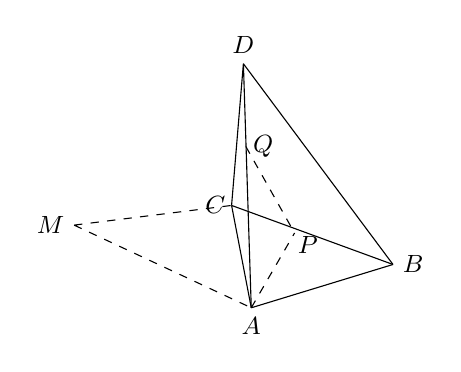
\begin{tikzpicture}[scale=1.0, font=\small]
  \coordinate (A) at (2.6,0);
  \coordinate (B) at (4.4,0.55);
  \coordinate (C) at (2.35,1.3);
  \coordinate (M) at (0.35,1.05);
  \coordinate (D) at (2.5,3.1);
  \coordinate (Q) at (2.53,2.05);
  \coordinate (P) at (3.15,0.95);
  \draw (A) -- (B);
  \draw (A) -- (C)  (B) -- (C);
  \draw (C) -- (D)  (A) -- (D);
  \draw (D) -- (B);
  \draw[dashed] (M) -- (A)  (M) -- (C);
  \draw[dashed] (A) -- (P)  (Q) -- (P);
  \node[below] at (A) {$A$};
  \node[right] at (B) {$B$};
  \node[left, inner sep=2pt] at (C) {$C$};
  \node[left] at (M) {$M$};
  \node[above] at (D) {$D$};
  \node[right, inner sep=2.5pt] at (Q) {$Q$};
  \node[below right, inner sep=1pt] at (P) {$P$};
\end{tikzpicture}
\end{center}
\nopagebreak[4]
  (1) 证明：平面 $ACD\perp$ 平面 $ABC$；

  (2) $Q$ 为线段 $AD$ 上一点，$P$ 为线段 $BC$ 上一点，且 $BP=DQ=\dfrac23DA$，求三棱锥 $Q\text{-}ABP$ 的体积。

\Needspace{4\baselineskip}
\textbf{解析}

\gksubpart{先算清折叠前后的所有长度}

平行四边形 $ABCM$ 中，$MC=AB=3$（对边相等），$AM=BC$（对边相等）。

在 $\mathrm{Rt}\triangle ACM$ 中（$\angle ACM=90^\circ$，$AC=MC=3$）：

\nopagebreak[4]
\[AM=\sqrt{3^{2}+3^{2}}=3\sqrt2\ \Longrightarrow\ BC=3\sqrt2\]

\textbf{折叠后}（$\triangle ACM$ 内部的量不变）：

\nopagebreak[4]
\[DC=MC=3,\qquad DA=MA=3\sqrt2,\qquad \angle ACD=\angle ACM=90^\circ\]

\gksubpart{(1) 证明平面 $ACD\perp$ 平面 $ABC$}

\textbf{第一步：找出底面内的垂直关系。}

在原平行四边形中 $AB\parallel MC$，而 $\angle ACM=90^\circ$ 说明 $MC\perp AC$，因此

\nopagebreak[4]
\[AB\perp AC\]

这条关系涉及的 $A$、$B$、$C$ \textbf{都在没有被折动的 $\triangle ABC$ 中}，所以折叠后依然成立。

\Needspace{0.25\textheight}

\textbf{第二步：与已知条件联立。}

已知 $AB\perp DA$。又 $AB\perp AC$，且

\nopagebreak[4]
\[AC\cap AD=A,\qquad AC,\ AD\subset\text{\text{平面} }ACD\]

由\textbf{线面垂直判定定理}：

\nopagebreak[4]
\[AB\perp\text{\text{平面} }ACD\]

\textbf{第三步：升级为面面垂直。}

$AB\subset$ 平面 $ABC$，过 $AB$ 的平面 $ABC$ 必与平面 $ACD$ 垂直：

\nopagebreak[4]
\[\text{\text{平面} }ACD\perp\text{\text{平面} }ABC\qquad\blacksquare\]

\Needspace{0.25\textheight}

\gksubpart{(2) 求三棱锥 $Q\text{-}ABP$ 的体积}

由 $DA=3\sqrt2$：

\nopagebreak[4]
\[BP=DQ=\frac23DA=\frac23\times3\sqrt2=2\sqrt2\]

注意 $BC=3\sqrt2$，故 $\dfrac{BP}{BC}=\dfrac{2\sqrt2}{3\sqrt2}=\dfrac23$；同样 $\dfrac{DQ}{DA}=\dfrac23$，即 $\dfrac{AQ}{AD}=\dfrac13$。

\textbf{建系}（由 (1) 已知 $AB\perp$ 平面 $ACD$，取 $AB$ 为竖直轴最方便）：

以 $A$ 为原点，平面 $ACD$ 为 $xOy$ 平面，$AB$ 方向为 $z$ 轴。

\begin{itemize}
\item $A(0,0,0)$，$C(3,0,0)$，$B(0,0,3)$。
\item 求 $D$：在 $\triangle ACD$ 中 $\angle ACD=90^\circ$，$AC=CD=3$，故 $\angle CAD=45^\circ$，$AD=3\sqrt2$。于是
\end{itemize}
\nopagebreak[4]
\[D\left(3\sqrt2\cos45^\circ,\ 3\sqrt2\sin45^\circ,\ 0\right)=(3,3,0)\]
\begin{itemize}
\item $Q$ 在 $AD$ 上且 $AQ=\dfrac13AD$：
\end{itemize}
\nopagebreak[4]
\[Q=\frac13D=(1,1,0)\]
\Needspace{0.25\textheight}

\begin{itemize}
\item $P$ 在 $BC$ 上且 $BP=\dfrac23BC$：
\end{itemize}
\nopagebreak[4]
\[P=B+\frac23\left(C-B\right)=(0,0,3)+\frac23(3,0,-3)=(2,0,1)\]

\textbf{算体积}：注意 $A$、$B$、$P$ 三点的 $y$ 坐标都是 $0$，即 $\triangle ABP$ 落在平面 $y=0$ 内。于是

\begin{itemize}
\item \textbf{点 $Q$ 到平面 $ABP$ 的距离} $=|y_Q|=1$；
\item \textbf{$\triangle ABP$ 的面积}：在 $xOz$ 平面内看，$A(0,0)$、$B(0,3)$、$P(2,1)$。边 $AB$ 在 $z$ 轴上、长为 $3$，点 $P$ 到 $z$ 轴的距离为 $2$：
\end{itemize}
\nopagebreak[4]
\[S_{\triangle ABP}=\frac12\times3\times2=3\]

\nopagebreak[4]
\[V_{Q\text{-}ABP}=\frac13\times S_{\triangle ABP}\times h=\frac13\times3\times1=1\]

\begin{gktip}
\textbf{方法提示}：翻折题一定要\textbf{先把"折叠中不变的量"逐条列出来}（本题是 $DC=3$、$DA=3\sqrt2$、$\angle ACD=90^\circ$），再用题目给的新条件（$AB\perp DA$）确定折起的角度。

第 (2) 问用坐标法比几何法稳：一旦发现 $\triangle ABP$ 恰在坐标平面内，"底面积 $\times$ 顶点的另一坐标"就直接出结果，省去找垂足的麻烦。
\end{gktip}

\gkanswer{答案（1）：见解析版}

\gkanswer{答案（2）：$V=1$}

\par\medskip

\end{answer}
\begin{answer}
\gksolhead{19}{12 分，频率分布与估计}

\textbf{题目}（12 分）：

某家庭记录了未使用节水龙头 $50$ 天的日用水量数据（单位：$\mathrm m^{3}$）和使用了节水龙头 $50$ 天的日用水量数据，得到频数分布表如下：

\textbf{未使用节水龙头 50 天的日用水量频数分布表}

\begin{center}
\begingroup\setlength{\tabcolsep}{4pt}
\begin{tabular}{cccccccc}
\toprule
日用水量 & $[0,0.1)$ & $[0.1,0.2)$ & $[0.2,0.3)$ & $[0.3,0.4)$ & $[0.4,0.5)$ & $[0.5,0.6)$ & $[0.6,0.7)$ \\
\midrule
频数 & $1$ & $3$ & $2$ & $4$ & $9$ & $26$ & $5$ \\
\bottomrule
\end{tabular}
\endgroup
\end{center}

\textbf{使用了节水龙头 50 天的日用水量频数分布表}

\begin{center}
\begin{tabular}{ccccccc}
\toprule
日用水量 & $[0,0.1)$ & $[0.1,0.2)$ & $[0.2,0.3)$ & $[0.3,0.4)$ & $[0.4,0.5)$ & $[0.5,0.6)$ \\
\midrule
频数 & $1$ & $5$ & $13$ & $10$ & $16$ & $5$ \\
\bottomrule
\end{tabular}
\end{center}

\Needspace{0.4\textheight}

  (1) 在答题卡上作出使用了节水龙头 $50$ 天的日用水量数据的频率分布直方图：
\nopagebreak[4]
\begin{center}% 2018 全国Ⅰ卷 文19：供作图用的空白频率分布直方图坐标网格
\begin{tikzpicture}
\begin{axis}[width=9.5cm, height=8cm, font=\small,
  xlabel={日用水量/$\mathrm{m}^{3}$}, ylabel={频率/组距},
  xlabel style={at={(1,0)}, anchor=west, font=\small},
  ylabel style={at={(0,1)}, anchor=south, rotate=-90, font=\small},
  xmin=0, xmax=0.65, ymin=0, ymax=3.5,
  xtick={0,0.1,...,0.6},
  ytick={0.2,0.4,...,3.4},
  yticklabel style={/pgf/number format/fixed, /pgf/number format/precision=1},
  xticklabel style={/pgf/number format/fixed, /pgf/number format/precision=1},
  grid=both, grid style={dashed, gray!45},
  axis lines=left, axis line style={-Stealth}]
\end{axis}
\end{tikzpicture}
\end{center}
\nopagebreak[4]
  (2) 估计该家庭使用节水龙头后，日用水量小于 $0.35\ \mathrm m^{3}$ 的概率；

  (3) 估计该家庭使用节水龙头后，一年能节省多少水？（一年按 $365$ 天计算，同一组中的数据以这组数据所在区间中点的值作代表。）

\Needspace{4\baselineskip}
\textbf{解析}

\gksubpart{(1) 作频率分布直方图}

频率分布直方图的\textbf{纵轴是"频率/组距"}，不是频率本身。这里组距为 $0.1$，样本容量 $50$，故

\nopagebreak[4]
\[\frac{\text{\text{频率}}}{\text{\text{组距}}}=\frac{\text{\text{频数}}/50}{0.1}=\frac{\text{\text{频数}}}5\]

使用了节水龙头的 $50$ 天数据换算如下：

\begin{center}
\begin{tabular}{ccccccc}
\toprule
日用水量 & $[0,0.1)$ & $[0.1,0.2)$ & $[0.2,0.3)$ & $[0.3,0.4)$ & $[0.4,0.5)$ & $[0.5,0.6)$ \\
\midrule
频数 & $1$ & $5$ & $13$ & $10$ & $16$ & $5$ \\
频率 & $0.02$ & $0.10$ & $0.26$ & $0.20$ & $0.32$ & $0.10$ \\
\textbf{频率/组距} & $\mathbf{0.2}$ & $\mathbf{1.0}$ & $\mathbf{2.6}$ & $\mathbf{2.0}$ & $\mathbf{3.2}$ & $\mathbf{1.0}$ \\
\bottomrule
\end{tabular}
\end{center}

按上表在给定网格中画出六个矩形即可（各矩形面积之和为 $0.02+0.10+0.26+0.20+0.32+0.10=1$ ）。

\gksubpart{(2) 估计日用水量小于 $0.35\ \mathrm m^{3}$ 的概率}

$0.35$ 落在 $[0.3,0.4)$ 这一组的\textbf{正中间}，按频率分布直方图的假设（\textbf{每组内数据均匀分布}），该组中有一半的天数小于 $0.35$：

\begin{itemize}
\item $[0,0.3)$ 三组共 $1+5+13=19$ 天（全部小于 $0.35$）；
\item $[0.3,0.35)$ 约占该组的一半：$\dfrac{10}2=5$ 天。
\end{itemize}

\nopagebreak[4]
\[P=\frac{19+5}{50}=\frac{24}{50}=0.48\]

\gksubpart{(3) 估计一年能节省多少水}

\textbf{用组中值算两组数据的日均用水量。}

\textbf{未使用节水龙头}（组中值依次为 $0.05,0.15,\cdots,0.65$）：

\nopagebreak[4]
\[\bar x_1=\frac{1\times0.05+3\times0.15+2\times0.25+4\times0.35+9\times0.45+26\times0.55+5\times0.65}{50}\]

分子逐项：$0.05+0.45+0.50+1.40+4.05+14.30+3.25=24.00$

\nopagebreak[4]
\[\bar x_1=\frac{24}{50}=0.48\ \left(\mathrm m^{3}\right)\]

\textbf{使用了节水龙头}：

\nopagebreak[4]
\[\bar x_2=\frac{1\times0.05+5\times0.15+13\times0.25+10\times0.35+16\times0.45+5\times0.55}{50}\]

分子逐项：$0.05+0.75+3.25+3.50+7.20+2.75=17.50$

\nopagebreak[4]
\[\bar x_2=\frac{17.5}{50}=0.35\ \left(\mathrm m^{3}\right)\]

\textbf{每天节省}：

\nopagebreak[4]
\[0.48-0.35=0.13\ \left(\mathrm m^{3}\right)\]

\textbf{一年节省}：

\nopagebreak[4]
\[0.13\times365=47.45\ \left(\mathrm m^{3}\right)\]

\begin{gktip}
\textbf{方法提示}：这类统计题的三个固定套路是"\textbf{纵轴是频率/组距}""\textbf{组内均匀分布}""\textbf{用组中值代替原始数据算平均}"。计算平均数时，把分子的七个乘积逐个列出再相加，比一次性心算更不容易出错 —— 这一步错一个数，第 (3) 问就全废了。
\end{gktip}

\gkanswer{答案（1）：频率/组距依次为 $0.2,\ 1.0,\ 2.6,\ 2.0,\ 3.2,\ 1.0$}

\gkanswer{答案（2）：$0.48$}

\gkanswer{答案（3）：约 $47.45\ \mathrm m^{3}$}

\par\medskip

\end{answer}
\begin{answer}
\gksolhead{20}{12 分，抛物线与角相等}

\textbf{题目}（12 分）：

设抛物线 $C:y^{2}=2x$，点 $A(2,0)$，$B(-2,0)$，过点 $A$ 的直线 $l$ 与 $C$ 交于 $M$，$N$ 两点。

  (1) 当 $l$ 与 $x$ 轴垂直时，求直线 $BM$ 的方程；

  (2) 证明：$\angle ABM=\angle ABN$。

\Needspace{4\baselineskip}
\textbf{解析}

\gksubpart{(1) 当 $l$ 与 $x$ 轴垂直时，求直线 $BM$ 的方程}

$l:x=2$ 代入 $y^{2}=2x$：

\nopagebreak[4]
\[y^{2}=4\ \Longrightarrow\ y=\pm2\]

取 $M(2,2)$（另一种取法对称）：

\nopagebreak[4]
\[k_{BM}=\frac{2-0}{2-(-2)}=\frac12\]

直线 $BM$：

\nopagebreak[4]
\[y=\frac12(x+2),\quad\text{\text{即}}\quad x-2y+2=0\]

若取 $M(2,-2)$，则得 $y=-\dfrac12(x+2)$。

\gksubpart{(2) 证明 $\angle ABM=\angle ABN$}

\textbf{转化}：$A$、$B$ 都在 $x$ 轴上，两角相等 $\iff$ $BM$ 与 $BN$ 关于 $x$ 轴对称 $\iff$

\nopagebreak[4]
\[k_{BM}+k_{BN}=0\]

\textbf{设直线的技巧}：因为 $l$ 过 $A(2,0)$ 且可能与 $x$ 轴垂直，若设 $y=k(x-2)$ 就要额外讨论斜率不存在的情形。改设

\nopagebreak[4]
\[l:x=my+2\]

这个形式\textbf{涵盖了所有过 $A$ 且不与 $x$ 轴重合的直线}（$m=0$ 即垂直情形），一次性避开分类讨论。

代入 $y^{2}=2x$：

\nopagebreak[4]
\[y^{2}=2(my+2)\ \Longrightarrow\ y^{2}-2my-4=0\]

设 $M\left(x_1,y_1\right)$、$N\left(x_2,y_2\right)$，韦达定理：

\nopagebreak[4]
\[y_1+y_2=2m,\qquad y_1y_2=-4\]

（判别式 $\Delta=4m^{2}+16>0$ 恒成立，两交点必存在。）

\textbf{计算斜率之和}。注意 $x_i+2=\left(my_i+2\right)+2=my_i+4$：

\nopagebreak[4]
\[k_{BM}+k_{BN}=\frac{y_1}{x_1+2}+\frac{y_2}{x_2+2}=\frac{y_1}{my_1+4}+\frac{y_2}{my_2+4}\]

通分，分子为

\nopagebreak[4]
\[y_1\left(my_2+4\right)+y_2\left(my_1+4\right)=2my_1y_2+4\left(y_1+y_2\right)\]

代入韦达定理：

\nopagebreak[4]
\[=2m\times(-4)+4\times2m=-8m+8m=0\]

分子恒为 $0$（与 $m$ 无关），而分母 $\left(my_1+4\right)\left(my_2+4\right)\ne0$（否则 $M$ 或 $N$ 与 $B$ 横坐标相同，但抛物线上 $x\ge0$，不可能等于 $-2$）。故

\nopagebreak[4]
\[k_{BM}+k_{BN}=0\]

即 $BM$ 与 $BN$ 的倾斜角互补，$\angle ABM=\angle ABN$。$\blacksquare$

\begin{gktip}
\textbf{方法提示}：\textbf{过定点且与 $x$ 轴不重合的直线，设成 $x=my+n$ 的形式}，是圆锥曲线大题中极其实用的技巧 —— 尤其当曲线是"横放"的抛物线 $y^{2}=2px$ 时，代入后直接得到关于 $y$ 的二次方程，韦达定理的形式最简洁。

点 $B(-2,0)$ 的来历也不是随意的：$A(2,0)$ 与 $B(-2,0)$ 关于原点对称，而抛物线 $y^{2}=2x$ 的准线是 $x=-\dfrac12$ —— 本题实际上是"过 $x$ 轴上一点的弦，从其关于原点的对称点看去张角相等"这一性质的实例。
\end{gktip}

\gkanswer{答案（1）：$y=\pm\dfrac12(x+2)$}

\gkanswer{答案（2）：见解析版}

\par\medskip

\end{answer}
\begin{answer}
\gksolhead{21}{12 分，导数}

\textbf{题目}（12 分）：

已知函数 $f(x)=a\mathrm e^{x}-\ln x-1$。

  (1) 设 $x=2$ 是 $f(x)$ 的极值点，求 $a$，并求 $f(x)$ 的单调区间；

  (2) 证明：当 $a\ge\dfrac1{\mathrm e}$ 时，$f(x)\ge0$。

\Needspace{4\baselineskip}
\textbf{解析}

\gksubpart{(1) 设 $x=2$ 是 $f(x)$ 的极值点，求 $a$ 并求单调区间}

\nopagebreak[4]
\[f'(x)=a\mathrm e^{x}-\frac1x\]

\textbf{由极值点定 $a$}：

\nopagebreak[4]
\[f'(2)=a\mathrm e^{2}-\frac12=0\ \Longrightarrow\ a=\frac1{2\mathrm e^{2}}\]

\textbf{代回并判断单调性}：

\nopagebreak[4]
\[f'(x)=\frac1{2\mathrm e^{2}}\mathrm e^{x}-\frac1x=\frac{\mathrm e^{x-2}}2-\frac1x\]

\textbf{关键观察}：在 $(0,+\infty)$ 上，$\dfrac{\mathrm e^{x-2}}2$ 单调递增，$-\dfrac1x$ 也单调递增（因为 $\dfrac1x$ 递减），\textbf{两个增函数之和仍是增函数}，故 $f'(x)$ 在 $(0,+\infty)$ 上\textbf{严格单调递增}。

又 $f'(2)=\dfrac{\mathrm e^{0}}2-\dfrac12=0$，所以 $x=2$ 是 $f'$ 的\textbf{唯一变号点}：

\begin{itemize}
\item $x\in(0,2)$ 时 $f'(x)<0$，$f$ \textbf{单调递减}；
\item $x\in(2,+\infty)$ 时 $f'(x)>0$，$f$ \textbf{单调递增}。
\end{itemize}

（这也验证了 $x=2$ 确实是极小值点。）

\gksubpart{(2) 证明：当 $a\ge\dfrac1{\mathrm e}$ 时，$f(x)\ge0$}

\textbf{第一步：放缩，把参数消掉。}

因 $\mathrm e^{x}>0$，当 $a\ge\dfrac1{\mathrm e}$ 时

\nopagebreak[4]
\[f(x)=a\mathrm e^{x}-\ln x-1\ \ge\ \frac1{\mathrm e}\mathrm e^{x}-\ln x-1=\mathrm e^{x-1}-\ln x-1\]

于是只需证明右边这个\textbf{不含参数}的函数非负。令

\nopagebreak[4]
\[g(x)=\mathrm e^{x-1}-\ln x-1,\qquad x>0\]

\textbf{第二步：求 $g$ 的最小值。}

\nopagebreak[4]
\[g'(x)=\mathrm e^{x-1}-\frac1x\]

与 (1) 同理，$\mathrm e^{x-1}$ 与 $-\dfrac1x$ 都在 $(0,+\infty)$ 上递增，故 $g'$ \textbf{严格递增}。又

\nopagebreak[4]
\[g'(1)=\mathrm e^{0}-1=1-1=0\]

所以：

\begin{itemize}
\item $x\in(0,1)$ 时 $g'(x)<0$，$g$ 递减；
\item $x\in(1,+\infty)$ 时 $g'(x)>0$，$g$ 递增。
\end{itemize}

$x=1$ 是 $g$ 的\textbf{唯一极小值点，也是最小值点}：

\nopagebreak[4]
\[g_{\min}=g(1)=\mathrm e^{0}-\ln1-1=1-0-1=0\]

\textbf{第三步：收尾。}

\nopagebreak[4]
\[g(x)\ge0\ \Longrightarrow\ f(x)\ge g(x)\ge0\qquad\blacksquare\]

（等号仅当 $a=\dfrac1{\mathrm e}$ 且 $x=1$ 时同时取到。）

\begin{gktip}
\textbf{方法提示}：含参不等式恒成立的证明，\textbf{第一步永远是想办法把参数去掉} —— 本题用 $a\ge\dfrac1{\mathrm e}$ 直接放缩到最不利的情形 $a=\dfrac1{\mathrm e}$，问题就变成了一个确定函数的最值问题。

另一个反复出现的技巧是判断 $f'$ 的单调性：$\mathrm e^{x}$ 型加 $-\dfrac1x$ 型必然是增函数，所以 $f'$ 至多一个零点，一旦找到就能直接确定 $f$ 的"先减后增"结构，\textbf{完全不需要再求二阶导数}。
\end{gktip}

\par\medskip

\Needspace{0.4\textheight}

\gkanswer{答案（1）：$a=\dfrac1{2\mathrm e^{2}}$；减区间 $(0,2)$，增区间 $(2,+\infty)$}

\gkanswer{答案（2）：见解析版}

\par\medskip

\end{answer}
\gkpart{选考题（现行考纲已取消，仅存档）}

\begin{answer}
\gksolhead{22}{10 分，坐标系与参数方程}

\textbf{题目}（10 分）〔选修 4-4：坐标系与参数方程〕：

（\textbf{已取消}）

在直角坐标系 $xOy$ 中，曲线 $C_1$ 的方程为 $y=k|x|+2$。以坐标原点为极点，$x$ 轴正半轴为极轴建立极坐标系，曲线 $C_2$ 的极坐标方程为 $\rho^{2}+2\rho\cos\theta-3=0$。

  (1) 求 $C_2$ 的直角坐标方程；

  (2) 若 $C_1$ 与 $C_2$ 有且仅有三个公共点，求 $C_1$ 的方程。

\textbf{解析}（同理科卷第 22 题）

\gksubpart{(1) 求 $C_2$ 的直角坐标方程}

代入 $\rho^{2}=x^{2}+y^{2}$、$\rho\cos\theta=x$：

\nopagebreak[4]
\[x^{2}+y^{2}+2x-3=0\ \Longrightarrow\ (x+1)^{2}+y^{2}=4\]

圆心 $(-1,0)$，半径 $2$。

\gksubpart{(2) 求 $C_1$ 的方程}

$C_1$ 是顶点 $(0,2)$ 的两条射线。顶点到圆心距离 $\sqrt5>2$，在圆外；每支最多 $2$ 个交点，要凑三个只能是"一支相切、一支两交点"。

$k>0$（开口向上）时两支都远离圆，凑不出三点，故 $k<0$。设右支所在直线 $kx-y+2=0$ 与圆相切：

\nopagebreak[4]
\[\frac{|-k+2|}{\sqrt{k^{2}+1}}=2\ \Longrightarrow\ 3k^{2}+4k=0\ \Longrightarrow\ k=-\frac43\ (k=0\ \text{\text{舍}})\]

\textbf{验证}：切点 $\left(\dfrac35,\dfrac65\right)$ 横坐标非负，确在右支上；左支与圆的两交点 $x=\dfrac{-33\pm12\sqrt6}{25}\approx-0.14,\ -2.50$ 均为负，确在左支上。共 $3$ 个公共点 

\par\medskip

\Needspace{0.5\textheight}

\gkanswer{答案（1）：$(x+1)^{2}+y^{2}=4$}

\gkanswer{答案（2）：$y=-\dfrac43|x|+2$}

\end{answer}
\begin{answer}
\gksolhead{23}{10 分，不等式选讲}

\textbf{题目}（10 分）〔选修 4-5：不等式选讲〕：

（\textbf{已取消}）

已知 $f(x)=|x+1|-|ax-1|$。

  (1) 当 $a=1$ 时，求不等式 $f(x)>1$ 的解集；

  (2) 若 $x\in(0,1)$ 时不等式 $f(x)>x$ 成立，求 $a$ 的取值范围。

\par\medskip

\textbf{解析}（同理科卷第 23 题）

\gksubpart{(1) $a=1$ 时解 $f(x)>1$}

$f(x)=|x+1|-|x-1|$，分三段：

\begin{itemize}
\item $x<-1$：$f=-2$，不满足；
\item $-1\le x<1$：$f=2x>1\Rightarrow x>\dfrac12$，得 $\dfrac12<x<1$；
\item $x\ge1$：$f=2>1$ 恒成立。
\end{itemize}

\gksubpart{(2) 若 $x\in(0,1)$ 时 $f(x)>x$，求 $a$ 的范围}

$x\in(0,1)$ 时 $|x+1|=x+1$，不等式化为

\nopagebreak[4]
\[x+1-|ax-1|>x\iff|ax-1|<1\iff0<ax<2\]

\begin{itemize}
\item $ax>0$ 且 $x>0$ $\Rightarrow a>0$；
\item $ax<2$ 对所有 $x\in(0,1)$ 成立 $\Rightarrow a\le2$（开区间使 $a=2$ 可取）。
\end{itemize}

\par\medskip

\gkanswer{答案（1）：$\left(\dfrac12,+\infty\right)$}

\gkanswer{答案（2）：$(0,2]$}

\end{answer}